\documentclass[a4paper,12pt]{article}

\usepackage{graphicx}
\usepackage[force]{feynmp-auto}
\usepackage{bm}

\unitlength=1mm
\graphicspath{{figures/}}

\begin{document}

\vspace{2cm}
\begin{center}
  \LARGE\bf {The Charge Exchange Reaction} \boldsymbol{$dp \to (pp)n$}
\end{center}
V.V.~Glagolev$^{1}$, G.~Martinsk\'{a}$^{2}$, J.~Mu\v{s}insk\'{y}$^{1,2}$,
N.M.~Piskunov$^{1}$, J.~Urb\'{a}n$^{2}$

\bigskip
\small{
  \noindent
  $^{1}$Joint Institute for Nuclear Research,141980 Dubna,Russia \\
  $^{2}$University of P.J.\v{S}af\'{a}rik, Jesenn\'{a} 5, SK-04154 Ko\v{s}ice,
  Slovak Republic
}

\bigskip
\begin{abstract}
  \noindent
  The ratio of the differential cross section of the charge exchange reaction on
  the deuteron to that on the nucleon at small transferred momenta has been
  discussed in order to estimate the spin-dependent part of the $np \to pn$
  charge exchange amplitude.
\end{abstract}

\vspace{1cm}
\section {Introduction}
During the recent years the interest to obtain some information on the cross
section of the spin-dependent part of the $np \to pn$ scattering using the
$dp \to  (pp)n$ charge exchange reaction  has been renewed. This is partly
connected with the appearence of accelerated deuterons on  the JINR LHE
Nuclotron with energies over 1 GeV /nucleon. The original ideas of Pomeranchuk
and Chew~\cite{a1} are also discussed revisited  as they have been formalized by
Dean and other authors~\cite{a8}. These formulas have been derived under certain
assumptions namely relying on the validity of the impulse and closure
approximations. In the work by Lednicky and Lyuboshitz~\cite {a2} it has been
shown that at relativistic energies these assumptions are justified. Moreover
experimental investigations of final state interactions (FSI) showed that the
backward-forward asymmetries of the
$ cos \alpha = (\vec {p_s} \vec {q})/({|\vec q|  |\vec p_{s}|}) $ distributions
are very sensitive to FSI, where $ \vec {p_s} $ - is the momentum of the
spectator with respect to the deuteron frame, and $ \vec {q} $ - is the
three-dimensional momentum transfer from the incident nucleon to the scattered
one. In the works \cite {a3, a4} it has been shown that for the values of
$ \vert t\vert <0.1 (GeV/c)^{2} $ and spectator momenta
$ \vert{\vec {p_s}}\vert < 0.1 $ GeV/c the asymmetries caused by FSI are
practically absent what is well demonstrated for both charge retention and
charge exchange deuteron break-up channels in the Fig.~\ref {f_asym}. It is
important to stress the above mentioned absence of FSI when moving to higher
energies where experimental data on np-scattering are scarce.  In the region
above 1 GeV only the preliminary results of the Delta-Sigma group \cite {a5} are
known. In connection with the achievements of the polarisation research methods
at Dubna (Nuclotron) and Juelich (COSY) - the chance of restoring the amplitudes
and phases of the nucleon-nucleon scattering in the region of energies below and
above 1 GeV has significantly enhanced. Related to the above mentioned facts the
experimental data from the $dp \to (pp)n$ reaction obtained by hydrogen bubble
chamber and published in \cite {a6} are going to be critically reviewed.

\begin{figure}[hbp]
  \begin{center}
    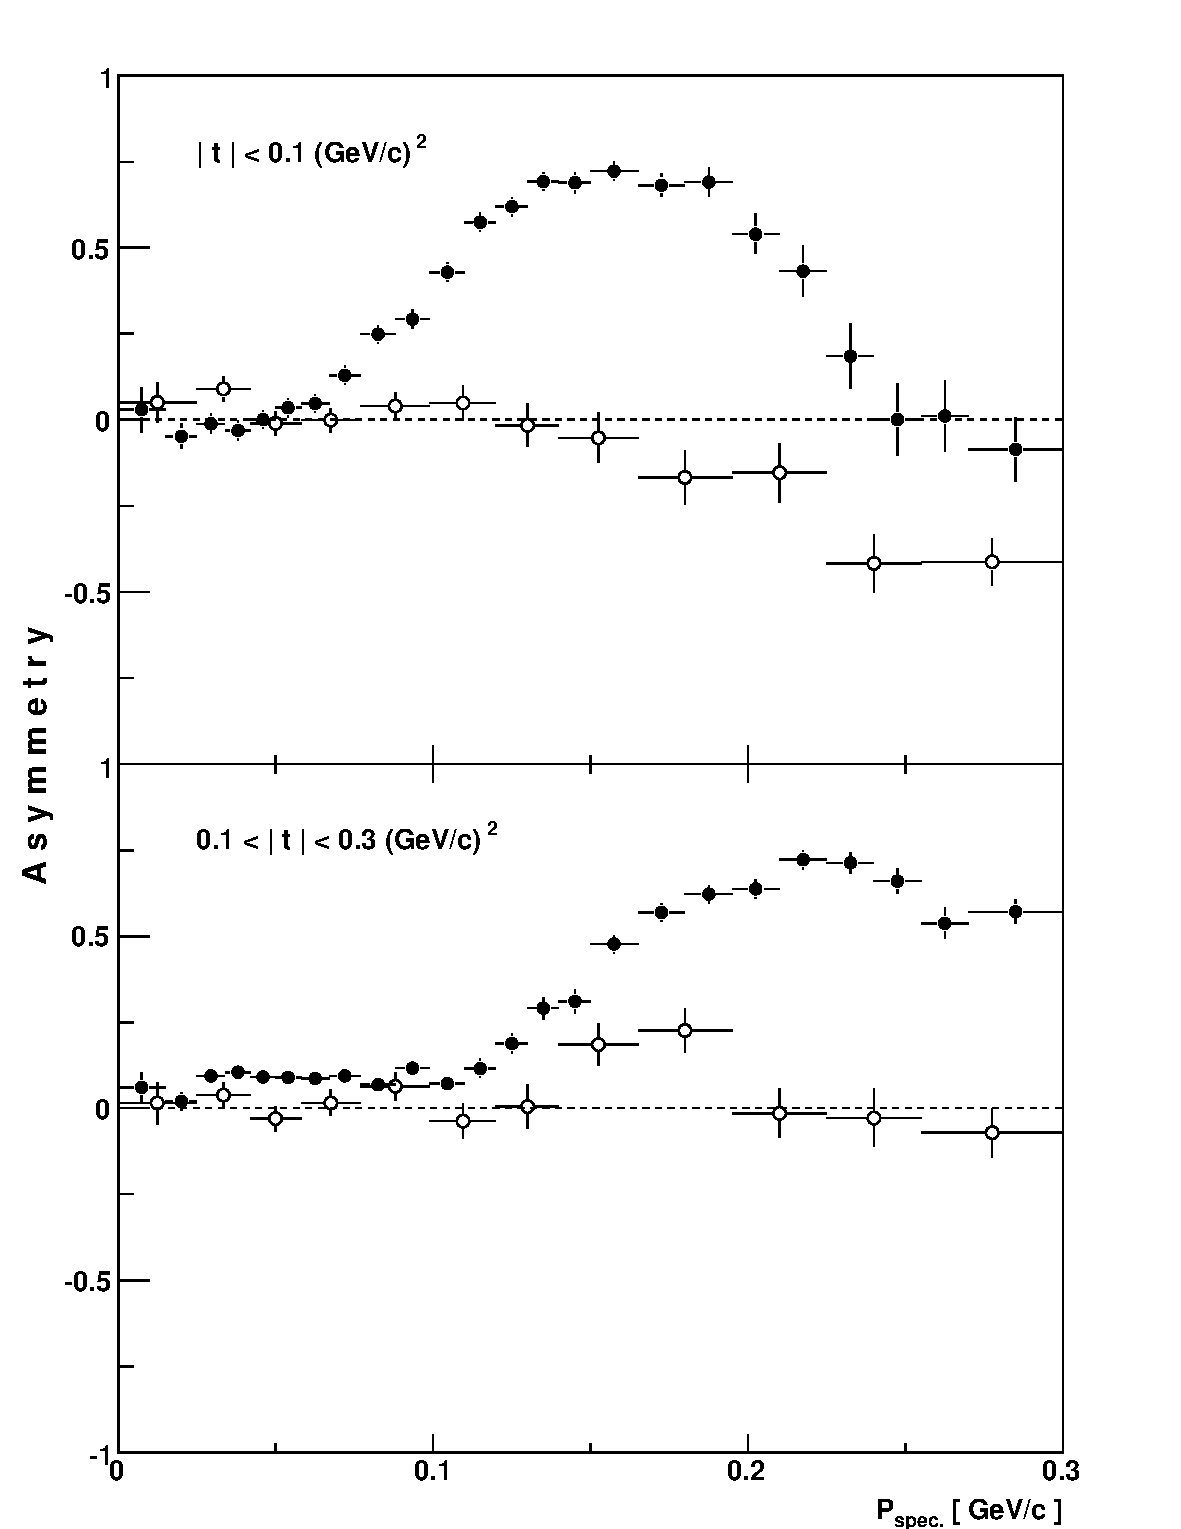
\includegraphics[angle=0,height=18cm]{fig_asym.pdf}
    \caption {Asymmetry of the angle
      $ cos \alpha = (\vec {p_s} \vec {q})/({|\vec q|  |\vec p_{s}|}) $ as a
      function of the spectator momenta $\vec{p_s}$. Symbol  $\vec{q}$ denotes
      the three momentum transfer from the incident nucleon to the scattered
      one. All the quantities are to be understood in the deuteron frame.  The
      empty circles correspond to charge exchange and full circles stand for the
      charge retention break-up data.}
    \label{f_asym}
  \end{center}
\end{figure}

\section{Experiment}
The experiment was realized on the JINR LHE synchrophasotron by means of the
one-metre hydrogen bubble  chamber irradiated with a deuteron beam of 3.35 GeV/c
momenta in full solid angle geometry. Applying the standard bubble chamber
processing chain: scanning, measuring, geometrical and kinematical
reconstruction and visual particle identification 17 reaction channels have been
observed. They are presented in Table 1. More detailed description of the
experimental set-up and data processing can be found in \cite {a16}.

\begin{table}[!hbp]
  \begin{center}
    \begin{tabular}{|r|l|r|} \hline &Channel&Number of events\\ \hline
      1.&$ppn$&102778\\ \hline 2.&$ppn\pi^{0}$&31295 \\ \hline
      3.&$p\pi^{+}nn$&65284 \\ \hline 4.&$dp$&16184\\ \hline
      5.&$dp\pi^{0}$&3950\\ \hline 6.&$dp\pi^{0}\pi^{0}$&1839\\ \hline
      7.&$d\pi^{+}n$&4963\\ \hline 8.&$d\pi^{+}n\pi^{0}$&1843\\ \hline
      9.&$\pi^{+}\pi^{+}nn$&315\\ \hline 10.&$ppp\pi^{-}$&5487\\
      \hline 11.&$ppp\pi{-}\pi^{0}$&167\\ \hline
      12.&$ppp\pi^{-}\pi^{0}\pi^{0}$&67\\ \hline
      13.&$pp\pi^{+}\pi^{-}n$&1163\\ \hline
      14.&$pp\pi^{+}\pi^{-}n\pi^{0}$&49\\ \hline
      15.&$dp\pi^{+}\pi^{-}$&576\\ \hline
      16.&$dp\pi^{+}\pi^{-}\pi^{0}$&39\\ \hline
      17.&$dp\pi^{+}\pi^{-}\pi^{0}\pi^{0}$&1414\\ \hline
    \end{tabular}
    \caption{The list of observed channels} \label{t_channels}
  \end{center}
\end{table}

Approximately half of the observed events corresponds to the deuteron pionless
break-up $dp \to ppn$ consisting of charge retention $dp \to (pn)p$  ~ 83 $\%$
and charge exchange $d p \to (pp)n$ reactions. In the latter case the neutron is
the fastest secondary nucleon in the deuteron frame and with 17 512 events,
equivalent to a cross section of 5.85$\pm$0.05 mb, forms about~17$\%$ of the
break-up. The millibarn equivalent per event was defined using the total dp
cross section \cite {a7} and corrections to the losses in dp-elastic channel at
small four-momenta transfers squared, defined as a transfer from the target
proton to the secondary neutron. The systematic error due to these losses was
about~4$\%$.

We recall briefly some of the theoretical formulas from ~\cite{a8,a9}. The
differential cross section of the elementary $pn \to np$ charge exchange process
may be represented as a sum of the spin-independent (subscript SI) and
spin-dependent (subscript SD) parts:

\begin{displaymath}
  (d\sigma/dt)_{np\rightarrow pn}=(d \sigma /dt)^{SI}_{np\rightarrow
    pn} + (d \sigma /dt)^{SD}_{np\rightarrow pn}
\end{displaymath}
The amplitude of the elementary $pn \to np$ charge-exchange reaction can be
written as:
\begin{displaymath}
  f_{ce}=a_{ce}+b_{ce} (\sigma \vec{n})( \sigma _{i}\vec{n})
  +c_{ce}[(\sigma \vec{n})+( \sigma _{i} \vec{n})]+d_{ce} [(\sigma
    \vec{m})( \sigma _{i}\vec{m})]+e_{ce} [(\sigma \vec{l})( \sigma
    _{i}\vec{l})],
\end{displaymath}
where the operators $\sigma$ and $\sigma_i$ are Pauli matrices of the incident
particle (neutron) and the ith nucleon (proton). The coefficients
$a_{ce}$, $b_{ce}$, $c_{ce}$, $d_{ce}$, $e_{ce}$ are complex functions of the
interacting particles energies and scattering angles. The quantities
$ \vec{n}, \vec {m} $ and $\vec{l} $ are defined as follows:
\begin{displaymath}
  \vec{n}=\frac{\vec{k}\times\vec{k'}}{|\vec{k}\times\vec{k'}|},~~
  \vec {m}=\frac{\vec{k'}-\vec{k}}{|\vec{k'}-\vec{k}|},~~
  \vec{l}=\frac{\vec{k'}+\vec{k}}{|\vec{k'}+\vec{k}|},
\end{displaymath}
where $ \vec{k}$  and $\vec{k'}$  are the  CMS incident and scattered nucleons
momenta. It is worth to stress that there are at least two space-time reflection
invariant representations of a scattering matrix (Goldberger~\cite{a10} and
Bystritsky, Lehar, Vinternic~ \cite{a11}), which are equivalent.

For the spin-independent and spin-dependent parts of differential cross section
we have:
\begin{displaymath}
  (d \sigma /dt)^{SI}_{np\rightarrow pn} = (\pi /p^{2}){\vert
  }a_{ce}{\vert }^{2}
\end{displaymath}
\begin{displaymath}
  (d \sigma /dt)^{SD}_{np\rightarrow pn} =(\pi/p^{2})[ \vert b_{ce}
    \vert ^{2}+ \vert c_{ce} \vert ^{2}+ \vert d_{ce} \vert ^{2}+ \vert
    e_{ce} \vert ^{2}],
\end{displaymath}
where p  is the momentum in the CM of NN-system.

The relation between the cross section of the peripheral charge exchange
$ dp \to ppn $ reaction on the deuteron and the elementary $pn \to  np$ one has
been discussed in many works. Mathematical formalism developed in~\cite{a8,a9}
allows to write the differential cross section for the deuteron charge-exchange
break-up reaction in the frame of the impulse approximation as follows:

\begin{displaymath}
  (d \sigma /dt)_{dp\rightarrow(pp)n} = [1-S(t)] (d \sigma
  /dt)^{SI}_{np\rightarrow pn} + [1-1/3S(t)] (d \sigma
  /dt)^{SD}_{np\rightarrow pn}.
\end{displaymath}
Here $S(t)= \int [\Psi(r)]^{2}e^{-iqr}d^{3}r$ denotes the deuteron form-factor,
$q^2 = t$ is the four-momentum transfer squared from the initial proton to the
neutron. This expression implies that at zero transfer from the target proton to
the neutron, i.e. at the scattering angle $180^{\circ}$ w.r.t. CMS and S(0) = 1,
the differential cross section equals to:

\begin{displaymath}
  (d \sigma /dt)_{dp\rightarrow(pp)n} = 2/3 (d \sigma
  /dt)^{SD}_{np\rightarrow pn}.
\end{displaymath}

Thus, the charge-exchange break-up reaction of the unpolarized deuteron on the
unpolarized target proton at zero transfer ($t = 0 $) is completely determined
by the spin-dependent part of the elementary $np \to pn$ backward scattering in
CMS ( $180^{\circ}$ ), so the deuteron acts as a spin filter. It should be noted
that this result also remains valid when the deuteron D-state is taken into
account~\cite{a2}. In the case of collinear kinematics
$\vert c_{ce}\vert ^2 = sin^2 \theta = 0$ and $\vert b_{ce}-e_{ce}\vert ^2 =
sin^2 \theta = 0$, that means for the backward scattering (charge exchange) one
obtains:
\begin{displaymath}
  (d \sigma /dt)_{dp\rightarrow(pp)n} = 2/3 (\pi/p^{2})[ 2\vert b_{ce}
    \vert ^{2}+ \vert d_{ce} \vert ^{2}].
\end{displaymath}
Thus, studying of process $dp \to (pp) n $ at small transferred momenta allows
to estimate the spin-dependent part of the elementary $np \to pn $ reactions,
i.e. the sum of the amplitudes
$2 \vert b _ {ce} \vert ^2 + \vert d _ {ce} \vert ^2 $.
\begin{figure}[!hbp]
  \begin{center}
    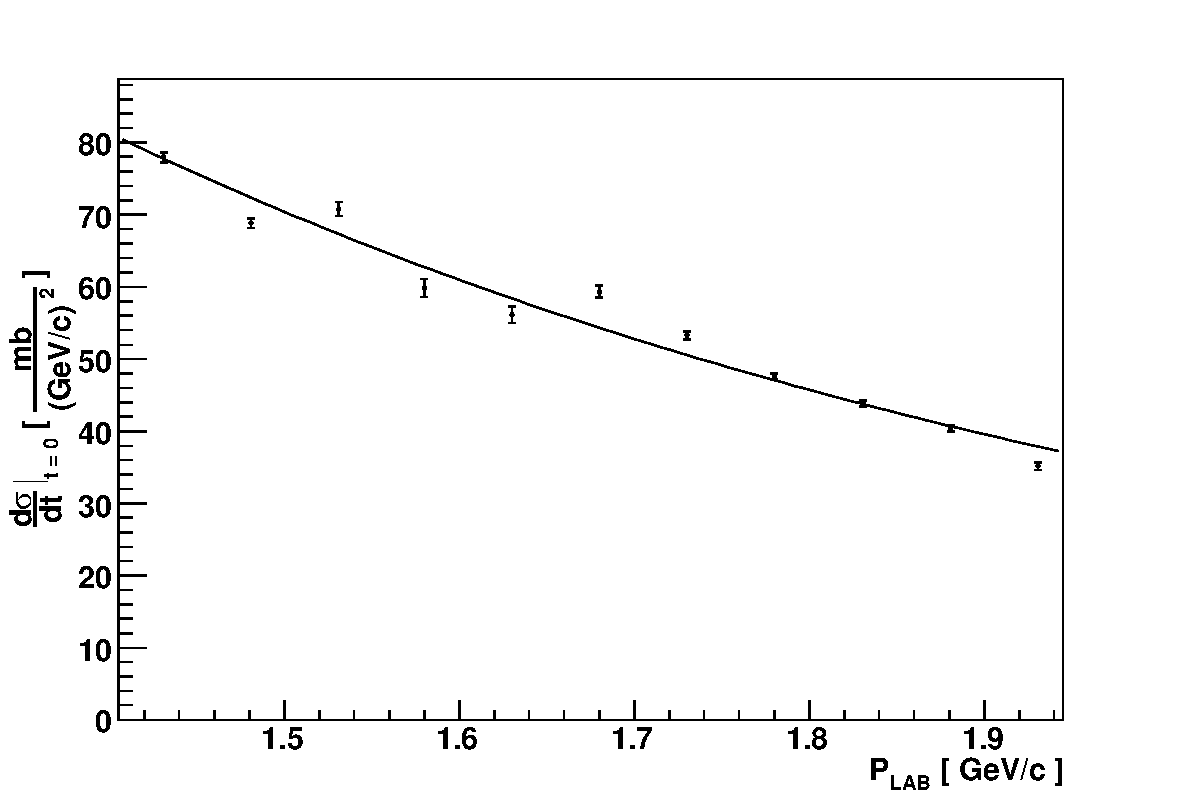
\includegraphics[angle=0,height=6cm, width=10cm]{fig_bizard.pdf}
    \caption {Extrapolation of the differential cross section from~\cite{a12}
      to $t=0$.}
    \label{f_biz}
  \end{center}
\end{figure}

The charge exchange differential cross section on the deuteron at $ t=0 $ will
be estimated from our data and compared with the available data for the
$ np \to pn $ reaction at the same energy. The nearest energy data come from the
measurements on SATURN accelerator ~\cite{a12,a13}. We would like to add that in
earlier publication \cite {a6} our data have been compared with that
of~\cite{a17}, where the cross section has been underestimated.

Fig.~\ref{f_biz} shows the results of differential cross sections on
$ np \to pn $ scattering taken from Bizard et al.~\cite{a12} in the region of
momenta $ (1.4 - 1.95) $ GeV/c extrapolated to $t = 0 $ by the expression
\begin{displaymath}
  d\sigma/dt = a \exp(bt+ct^2).
\end{displaymath}

The exponential fit to these values  gives for our incident momentum of  1.675
GeV/c/nucleon the following value $d \sigma/dt | _ {t=0} = 54.7 \pm 0.2$
mb /(GeV/c)$^{2}$. To the received value we will refer later and  the estimated
differential cross section of the quasi-elastic $dp \to (pp) n $ charge-exchange
at $t = 0 $ will be compared to. One would like to stress that the systematic
error in data by Bizard et al.~\cite{a12} makes $5\%$.

\begin{figure}[!hbp]
  \begin{center}
    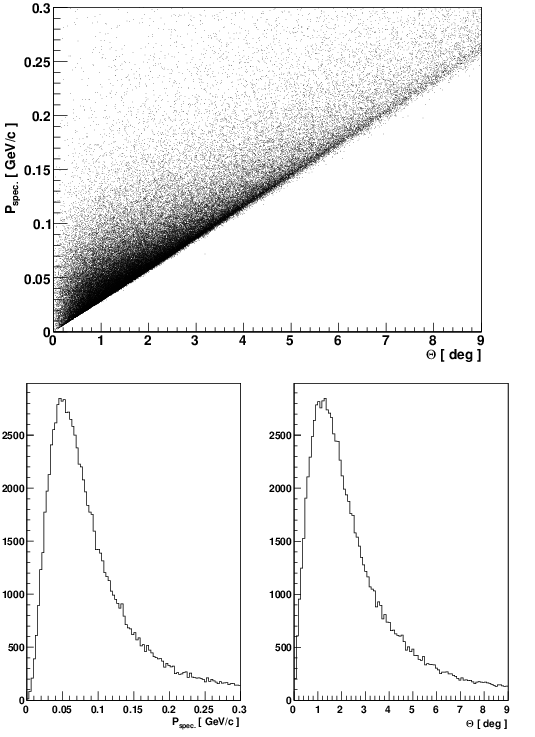
\includegraphics[angle=0,height=12.5cm,width=11cm]{fig_theta_p.png}
    \caption { Nucleon-spectator momentum (in the deuteron frame) dependence on
      its polar angle (in the target proton frame). The diagrams below  are the
      projections to axes.}
    \label{f_tp}
  \end{center}
\end{figure}

From the kinematical correlation between the polar angle of the
nucleon-spectator (in the laboratory frame) and its momentum (in the deuteron
rest frame) shown in the Fig.~\ref{f_tp} one can see the enhanced population
of events at the angles below~$5 ^{\circ}$. This sample is enriched with events
corresponding to quasi-nucleon scattering. In the case of $t = 0 $ both  protons
in the laboratory frame have practically identical momenta
$ \vec {p} _1 = \vec {p} _2 = (1/2) \vec {p} _d $. For the set of proton pairs
within the cone of $ 5 ^{\circ} $ the $d \sigma/dt $ distribution is
histogrammed and weighted  with the millibarn equivalent and a correction factor
for the flux, equal to the ratio of total number of nucleon-spectator to the
number of spectators in this cone.

In connection with the appreciable contribution of events with intermediate
$ \Delta $-isobar \cite{a14, a4}, the main part of which comes from quasi-pp
collisions (proceeding mainly via $ \Delta ^{++} $ and $ \Delta ^{+} $-isobars)
see diagrams a) and b) in the Fig.~\ref{f_feynman}, it would be necessary to
introduce a correction for this effect.
\\ \\

\begin{figure}[!hbp]
  \begin{center}

    \begin{fmffile}{ppn_fmf}
      % pp1
      \parbox{56mm} {
        \begin{fmfgraph*}(54,27)
          \fmfset{arrow_len}{4mm}\fmfset{arrow_ang}{8}

          \fmfleft{iA,iB}
          \fmfright{o1,o2,o3}
          \fmflabel{$d$}{iA}
          \fmflabel{$p$}{iB}
          \fmflabel{$p$}{o3}
          \fmflabel{$n$}{o2}
          \fmflabel{$p$}{o1}

          \fmf{fermion,tension=1.0}{iA,v1} % default tension=1.0
          \fmf{fermion,tension=1.0}{v2,o1}
          \fmf{fermion,tension=1.0}{v2,o2}
          \fmf{fermion,tension=1.0}{iB,v3,o3}

          \fmf{fermion,tension=1.5,label=$n$}{v1,v2}
          \fmf{fermion,tension=0.2,lab.side=left,label=$p$}{v1,v3}
          \fmf{fermion,tension=0.1,lab.side=left,label=$\Delta^{+}$}{v3,v2}

          \fmfblob{0.06w}{v1}
          \fmfdot{v2,v3}
          \fmf{dbl_plain_arrow}{iA,v1}
          \fmffreeze
          \fmf{dbl_plain_arrow}{v3,v2}

        \end{fmfgraph*}
      }
      % pp2
      \quad
      \parbox{56mm} {
        \begin{fmfgraph*}(54,27)
          \fmfset{arrow_len}{4mm}\fmfset{arrow_ang}{8}

          \fmfleft{iA,iB}
          \fmfright{o1,o2,o3}
          \fmflabel{$d$}{iA}
          \fmflabel{$p$}{iB}
          \fmflabel{$n$}{o3}
          \fmflabel{$p$}{o2}
          \fmflabel{$p$}{o1}

          \fmf{fermion,tension=1.0}{iA,v1} % default tension=1.0
          \fmf{fermion,tension=1.0}{v2,o1}
          \fmf{fermion,tension=1.0}{v2,o2}
          \fmf{fermion,tension=1.0}{iB,v3,o3}

          \fmf{fermion,tension=1.5,label=$n$}{v1,v2}
          \fmf{fermion,tension=0.2,lab.side=left,label=$p$}{v1,v3}
          \fmf{fermion,tension=0.1,lab.side=left,label=$\Delta^{++}$}{v3,v2}

          \fmfblob{0.06w}{v1}
          \fmfdot{v2,v3}
          \fmf{dbl_plain_arrow}{iA,v1}
          \fmffreeze
          \fmf{dbl_plain_arrow}{v3,v2}
        \end{fmfgraph*}
      }
      \begin{center}
        %\vspace{5mm}
        \texttt{a)} \hspace{56mm} \texttt{b)}
      \end{center}
      % np1
      \vspace{10mm}
      \parbox{56mm} {
        \begin{fmfgraph*}(54,27)
          \fmfset{arrow_len}{4mm}\fmfset{arrow_ang}{8}

          \fmfleft{iA,iB}
          \fmfright{o1,o2,o3}
          \fmflabel{$d$}{iA}
          \fmflabel{$p$}{iB}
          \fmflabel{$n$}{o3}
          \fmflabel{$p$}{o2}
          \fmflabel{$p$}{o1}

          \fmf{fermion,tension=1.0}{iA,v1} % default tension=1.0
          \fmf{fermion,tension=1.0}{v2,o1}
          \fmf{fermion,tension=1.0}{v2,o2}
          \fmf{fermion,tension=1.0}{iB,v3,o3}

          \fmf{fermion,tension=1.5,label=$p$}{v1,v2}
          \fmf{fermion,tension=0.2,lab.side=left,label=$n$}{v1,v3}
          \fmf{fermion,tension=0.1,lab.side=left,label=$\Delta^{+}$}{v3,v2}

          \fmfblob{0.06w}{v1}
          \fmfdot{v2,v3}
          \fmf{dbl_plain_arrow}{iA,v1}
          \fmffreeze
          \fmf{dbl_plain_arrow}{v3,v2}

        \end{fmfgraph*}
      }
      % pp2
      \quad
      \parbox{56mm} {
        \begin{fmfgraph*}(54,27)
          \fmfset{arrow_len}{4mm}\fmfset{arrow_ang}{8}

          \fmfleft{iA,iB}
          \fmfright{o1,o2,o3}
          \fmflabel{$d$}{iA}
          \fmflabel{$p$}{iB}          \fmflabel{$p$}{o3}
          \fmflabel{$n$}{o2}
          \fmflabel{$p$}{o1}

          \fmf{fermion,tension=1.0}{iA,v1} % default tension=1.0
          \fmf{fermion,tension=1.0}{v2,o1}
          \fmf{fermion,tension=1.0}{v2,o2}
          \fmf{fermion,tension=1.0}{iB,v3,o3}
          \fmf{fermion,tension=1.5,label=$p$}{v1,v2}
          \fmf{fermion,tension=0.2,lab.side=left,label=$n$}{v1,v3}
          \fmf{fermion,tension=0.1,lab.side=left,label=$\Delta^{\circ}$}{v3,v2}

          \fmfblob{0.06w}{v1}
          \fmfdot{v2,v3}
          \fmf{dbl_plain_arrow}{iA,v1}
          \fmffreeze
          \fmf{dbl_plain_arrow}{v3,v2}

        \end{fmfgraph*}
      }
      \begin{center}
        %\vspace{5mm}
        \texttt{c)} \hspace{56mm} \texttt{d)}
      \end{center}
    \end{fmffile}

    \caption{The Feynman diagrams for $dp\rightarrow ppn$ reactions with
      intermediate $\Delta$-isobar.}
    \label{f_feynman}
  \end{center}
\end{figure}

In the Fig.~\ref{f_res} the comparison of the spectator momenta distributions
from the charge retention and charge exchange break-ups is shown. The relative
enhancement in the spectrum of the proton spectators from the charge exchange,
connected with the contribution intermediate isobaric states, is clearly
visible. Comparing the two-dimensional plot in Fig.~\ref{f_tp} with the
histogram in the Fig.~ \ref {f_res} one can see that this enhancement is
concentrated in the region of momenta above 0.2 GeV/c, i.e. outside the cone of
$5 ^{\circ}$ and does not influence the differential cross section at $t = 0 $.

The results of an exponential fit to the differential cross section,
approximated in the same way as for the  $np \to pn $ data, is shown in the
Fig.~\ref{f_2p}. The extrapolation to $t = 0$ has given a value of
$ d \sigma/dt\vert_{t=0}$ = $30.2 \pm 4.1$ mb/$(GeV/c)^{2}$.

\begin{figure}[!hbp]
  \begin{center}
    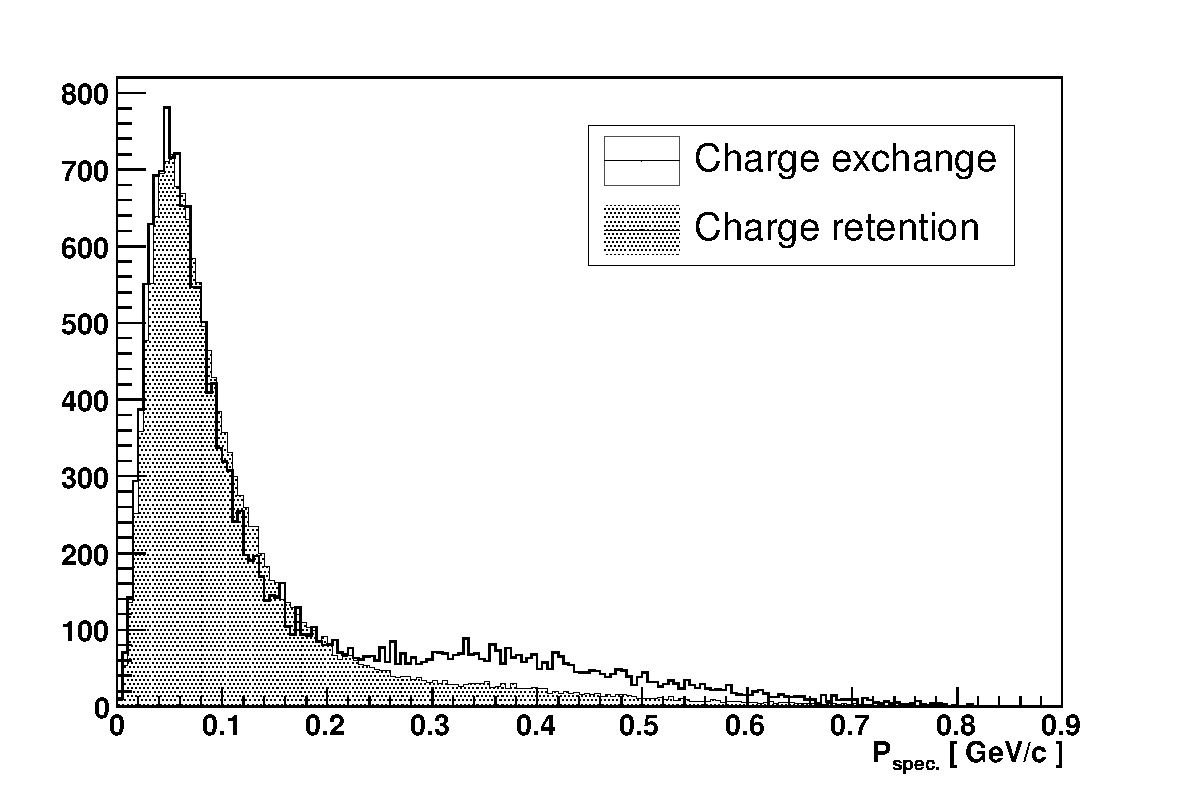
\includegraphics[angle=0,height=8cm]{fig_res.pdf}
    \caption { Spectator momentum distributions from the charge retention and
      charge exchange channels normalized to the  maxima.} \label {f_res}
  \end{center}
\end{figure}

One can introduce the ratio of the differential cross sections at $t = 0 $
for the forward scattering (charge exchange) on the deuteron and proton
$R = \frac {(d \sigma/dt) _ {dp}} {(d \sigma/dt) _ {np}} = 0.55 \pm 0.08 $.
Under the assumptions stated above it can be related to
$\frac {2} {3} \times \frac {(d \sigma/dt) _ {np}^ {SD}} {(d \sigma/dt) _ {dp}}$
and accordingly the value of the spin-independent part of the elastic
$np \to pn $ charge exchange  cross section $R^{ID}_{np} = \frac {(d \sigma/dt) _
  {np}^{SI}} {(d \sigma/dt)_{np}^{SD}} = {\frac {2} {3 \times R} - 1} =
0.21 \pm 0.17$ has been obtained.

\begin{figure}[!htp]
  \begin{center}
    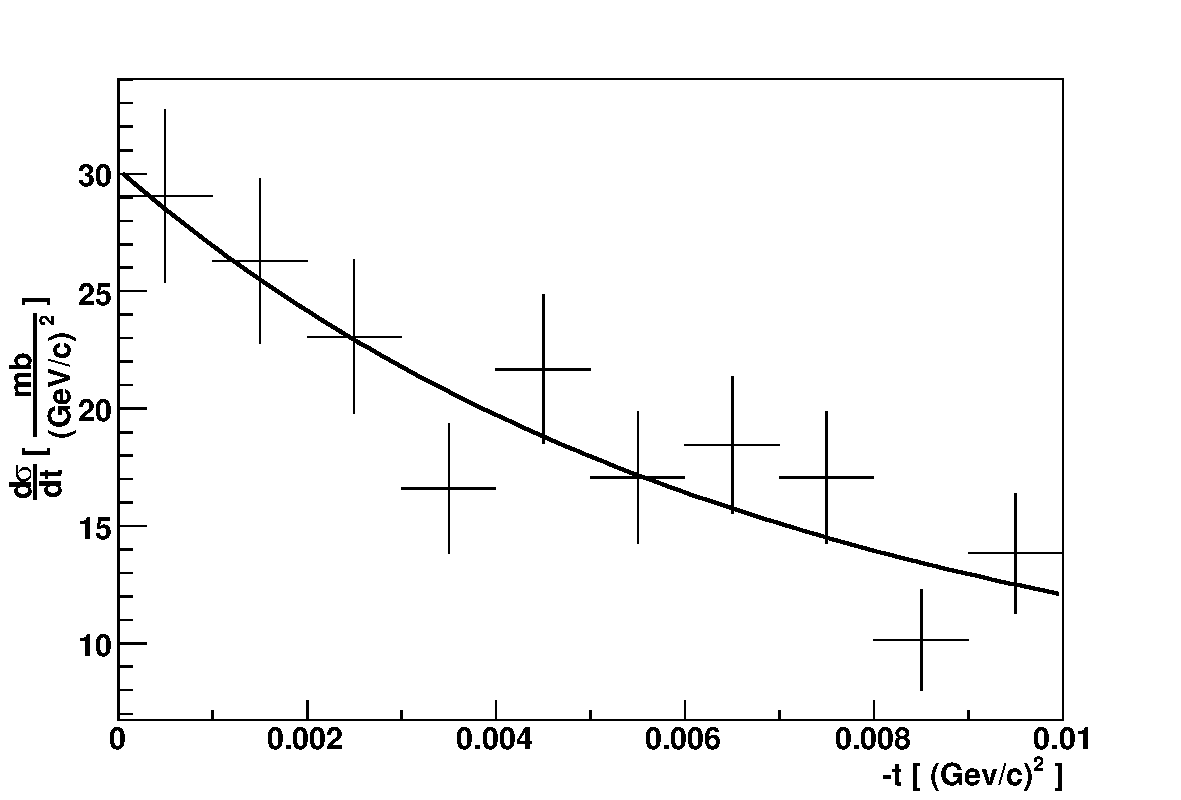
\includegraphics[angle=0,height=8cm]{fig_2p.pdf}
    \caption {Extrapolation of the differential cross section to $t = 0$.}
    \label{f_2p}
  \end{center}
\end{figure}

\section {Conclusion}
\begin{enumerate}
\item{ The representation of the experimental data from the $dp\to(p p)n$
  reaction, received by hydrogen bubble chamber, has been critically reviewed.}
\item{ The obtained ratio $R = 0.55\pm 0.08$ of the charge exchange differential
  cross section from the reaction $dp\to(pp)n$  to  that for the $n p\to p n$ at
  $t = 0$ testifies the prevailing contribution of the spin-dependent part to
  the $n p\to pn$ scattering amplitude.}
\item{Continuation of this research at higher energies is therefore desirable.}
\end{enumerate}

\section {Acknowledgements}
The authors are thankful to N.B.Ladygina, V.L.Lyuboshitz and F.Lehar for useful
discussions.
\\ \\
This work was supported under Slovak Grant Agency VEGA 1/4010/07.

\newpage
\begin {thebibliography} {99}
\bibitem{a1}I.Pomeranchuk, Sov. JETF {\bf 21}, 1113 (1951).\\
  G.F.Chew,Phys.Rev. {\bf 84}, 710 (1951).
\bibitem{a8}N.W.Dean, Phys.Rev. {\bf D5}, 1661 (1972).
\bibitem{a2}R.Lednicky,V.L.Lyuboshitz, V.V.Lyuboshitz, Proc. XVI ISHEPP, Dubna
  2004, 199.
\bibitem{a3}B.S.Aladashvili et al., J.Phys.G: Nucl.Phys. {\bf 3}, 7 (1977).
\bibitem{a4}B.S.Aladashvili et al., J.Phys.G: Nucl.Phys. {\bf 3}, 1225 (1977).
\bibitem{a5}V.I.Sharov et al., Czech.J.Phys. {\bf 55}, A283 (2005).
\bibitem{a6}V.V.Glagolev et al., Eur.Phys.J {\bf A15}, 471 (2002).
\bibitem{a9}D.Bugg,C.Wilkin, Nucl.Phys. {\bf A 467} 575 (1987).
\bibitem{a7}D.V.Bugg et al., Phys.Rev. {\bf 146}, 980 (1966).
\bibitem{a16} B.S.Aladashvili et al., NIM, {\bf 129}, 109 (1975).\\
  JINR Commun. 1-7645, Dubna, 1973.
\bibitem{a10}M.Goldberger, K.Watson, Collision Theory,Willey, New York (1966).
\bibitem{a11}J.Bystricky, F.Lehar and P.Winternitz,J.Phys. (Paris) {\bf 39}, 1
  (1978).
\bibitem{a12}G.Bizard et al., Nuclear Physics {\bf B85}, 14 (1975).
\bibitem{a13}J.Bystricky,F.Lehar,  Nucleon-Nucleon Scattering data,editors
  H.Behrens and G.Ebel, Fachinformationszentrum Karlsruhe,1978 Edition,N 11-1,
  p.521
\bibitem{a17}P.F.Shephard et al., Phys. Rev. {\bf D10}, 2735 (1974).
\bibitem{a14}B.S.Aladashvili et.al., Nucl.Phys. {\bf A274}, 486 (1976).
\end {thebibliography}
\end{document}
